\documentclass{article}

\usepackage{Engineering}
\usepackage{multicol}
\usepackage{tcolorbox}
\usepackage{titlesec}
\usepackage{titling}
\usepackage{etoolbox}
\usepackage{tabularx}

% === METADATA ===
\pdftitle{EFPLab1 Cheatsheet}

% === HEADER/FOOTER ===
\usepackage{fancyhdr}
\pagestyle{fancy}
\fancyhf{}
\lhead{Matteo Frongillo}
\chead{\nouppercase{\leftmark}}
\rhead{\thepage}

\renewcommand{\sectionmark}[1]{\markboth{#1}{}}

% === CUSTOM BOX COMMANDS ===
\definecolor{BoxBG}{HTML}{F0F8FF}
\definecolor{BoxBorder}{HTML}{3B83BD}

\newtcolorbox{theorybox}[1]{
  colback=BoxBG,
  colframe=BoxBorder,
  fonttitle=\bfseries,
  left=1mm,right=1mm,top=1mm,bottom=1mm,
  boxrule=0.8pt,
  arc=1.5mm,
  title={\begingroup\intheoryboxtitletrue #1\endgroup\intheoryboxtitlefalse}
}

\newtcolorbox{examplebox}[1]{
  colback=gray!10!white,
  colframe=gray!80!black,
  coltitle=white,
  fonttitle=\bfseries,
  left=1mm,right=1mm,top=1mm,bottom=1mm,
  boxrule=0.8pt,
  arc=1.5mm,
  title={#1}
}

\newtcolorbox{formula}[1]{
  colback=red!10!white,
  colframe=red!90!black!75,
  fonttitle=\bfseries,
  left=1mm,right=1mm,top=1mm,bottom=1mm,
  boxrule=0.8pt,
  arc=1.5mm,
  title={#1}
}

% === SECTION TITLE FORMATTING ===
\newif\ifintheoryboxtitle
\intheoryboxtitlefalse

\titleformat{\section}
  {\ifintheoryboxtitle\color{white}\else\color{BoxBorder}\fi\Large\bfseries}
  {\thesection}{0.5em}{}

\titleformat{\subsection}
  {\ifintheoryboxtitle\color{white}\else\color{BoxBorder}\fi\bfseries}
  {\thesubsection}{0.5em}{}

\titleformat{\subsubsection}
  {\ifintheoryboxtitle\color{white}\else\color{BoxBorder}\fi\small\bfseries}
  {\thesubsubsection}{0.5em}{}

% === DOCUMENT ===
\begin{document}
\begin{multicols}{2}
\setlength{\columnsep}{1pt}

% === CONTENT ===
\section{Preambule}
\begin{theorybox}{Theory box}
    Lorem ipsum dolor sit amet.
\end{theorybox}

\begin{formula}{Formula box}
    Lorem ipsum dolor sit amet.
\end{formula}

\begin{examplebox}{Lab/examples box}
    Lorem ipsum dolor sit amet.
\end{examplebox}

\section{Fluids as energy carriers}
\subsection{Fluid state variables and properties}

\begin{theorybox}{Formulas}
    \subsubsection{State variables}
    \textbf{Density}
    \begin{equation}
        \rho \triangleq \dfrac{m}{V} \left[\dfrac{kg}{m^3}\right] 
    \end{equation}

    \textbf{Specific volume}
    \begin{equation}
        v \triangleq \dfrac{V}{m} = \dfrac{1}{\rho} \left[\dfrac{m^3}{kg}\right]
    \end{equation}

    \subsubsection{Viscosity}
    \textbf{Kinematic viscosity}
    \begin{equation}
        \nu \triangleq \dfrac{\eta}{\rho} \left[\dfrac{m^2}{s}\right]
    \end{equation}

    \textbf{Dynamic viscosity}
    \begin{equation}
        \eta \triangleq \nu\cdot\rho \left[Pa\cdot s = \dfrac{Ns}{m^2} = \dfrac{kg}{m \cdot s}\right]
    \end{equation}

    \subsubsection{Real and ideal fluid}
    \begin{tabularx}{\linewidth}{@{}X@{\hspace{.1766cm}}X@{}}
        \textbf{Real fluid} & \textbf{Ideal fluid} \\
        variable density $\left(\Delta \rho \neq 0\right)$ & incompressible $\left(\Delta \rho = 0\right)$ \\
        friction $\left(\eta > 0, \nu > 0\right)$ & frictionless $\left(\eta=0, \nu=0\right)$ \\
    \end{tabularx}
    \\
    \subsubsection{Compressibility}
    \textbf{Mach number}
    \begin{equation}
        M \triangleq \dfrac{u}{c}
    \end{equation}
    where:
    \begin{itemize}
        \item $M$ is the Mach number [-]\\
            $M \lesssim 0.3$: incompressible flow
        \item $u$ is the flow velocity [m/s]
        \item $c$ is the speed of sound in the fluid [m/s]
    \end{itemize}
    and:
    \begin{itemize}
        \item $c_{\text{w}}^{20^\circ} = 1484$ m/s
        \item $c_{\text{a}}^{20^\circ} = 343$ m/s
    \end{itemize}
\end{theorybox}

\vfill
\phantom{}
\columnbreak

\subsection{Laminar and turbulent flow}
\begin{formula}{Reynolds number}
    \begin{equation}
        Re = \dfrac{v\cdot L}{\nu} = \dfrac{\rho\cdot v\cdot L}{\eta} \left[-\right]
    \end{equation}
    where:
    \begin{itemize}
        \item $v$ is the mean flow velocity [m/s]
        \item $L$ is the characteristic length [m]
    \end{itemize}
    \begin{examplebox}{Re values}
    \begin{itemize}
        \item $Re < 2000$: laminar flow
        \item $Re \simeq 2300$: critical point
        \item $2000 < Re < 4000$: transitional regime
        \item $Re \geq 4000$: turbulent flow
    \end{itemize}
    \end{examplebox}
\end{formula}

\subsection{Pressure and velocity}
\begin{theorybox}{Pressure}
    \subsubsection{Total pressure}
    Added to the static pressure $p_{\rm stat}$, there is also the
    dynamic pressure $p_{\rm dyn}$ and the total pressure $p_{\rm tot}$:
    \begin{equation}
        p_{\rm tot} = p_{\rm stat} + p_{\rm dyn} = \rho\left(gh + \frac{v^2}{2}\right)
    \end{equation}

    \subsubsection{Absolute pressure}
    Absolute pressure $p_{\rm abs}$ refers to the pressure in a vacuum
    $p_{\rm vaacum}=0$ Pa while relative pressure $p_{\rm rel}$ can refer to
    any chosen reference pressure $p_{\rm ref}$.
    \begin{equation}
        p_{\rm abs} = p_{\rm rel} - p_{\rm ref}
    \end{equation}

    \subsubsection{Velocity}
    Velocity is a vector quantity:
    \begin{equation}
        \vec{v} = \left(v_x v_y v_z\right)
    \end{equation}

    The magnitude is given by:
    \begin{equation}
        v = \sqrt{v_x^2 + v_y^2 + v_z^2}
    \end{equation}
\end{theorybox}

\subsection{Curvature pressure formula}
\begin{examplebox}{Deflection motion of a fluid element around a blunt body}
    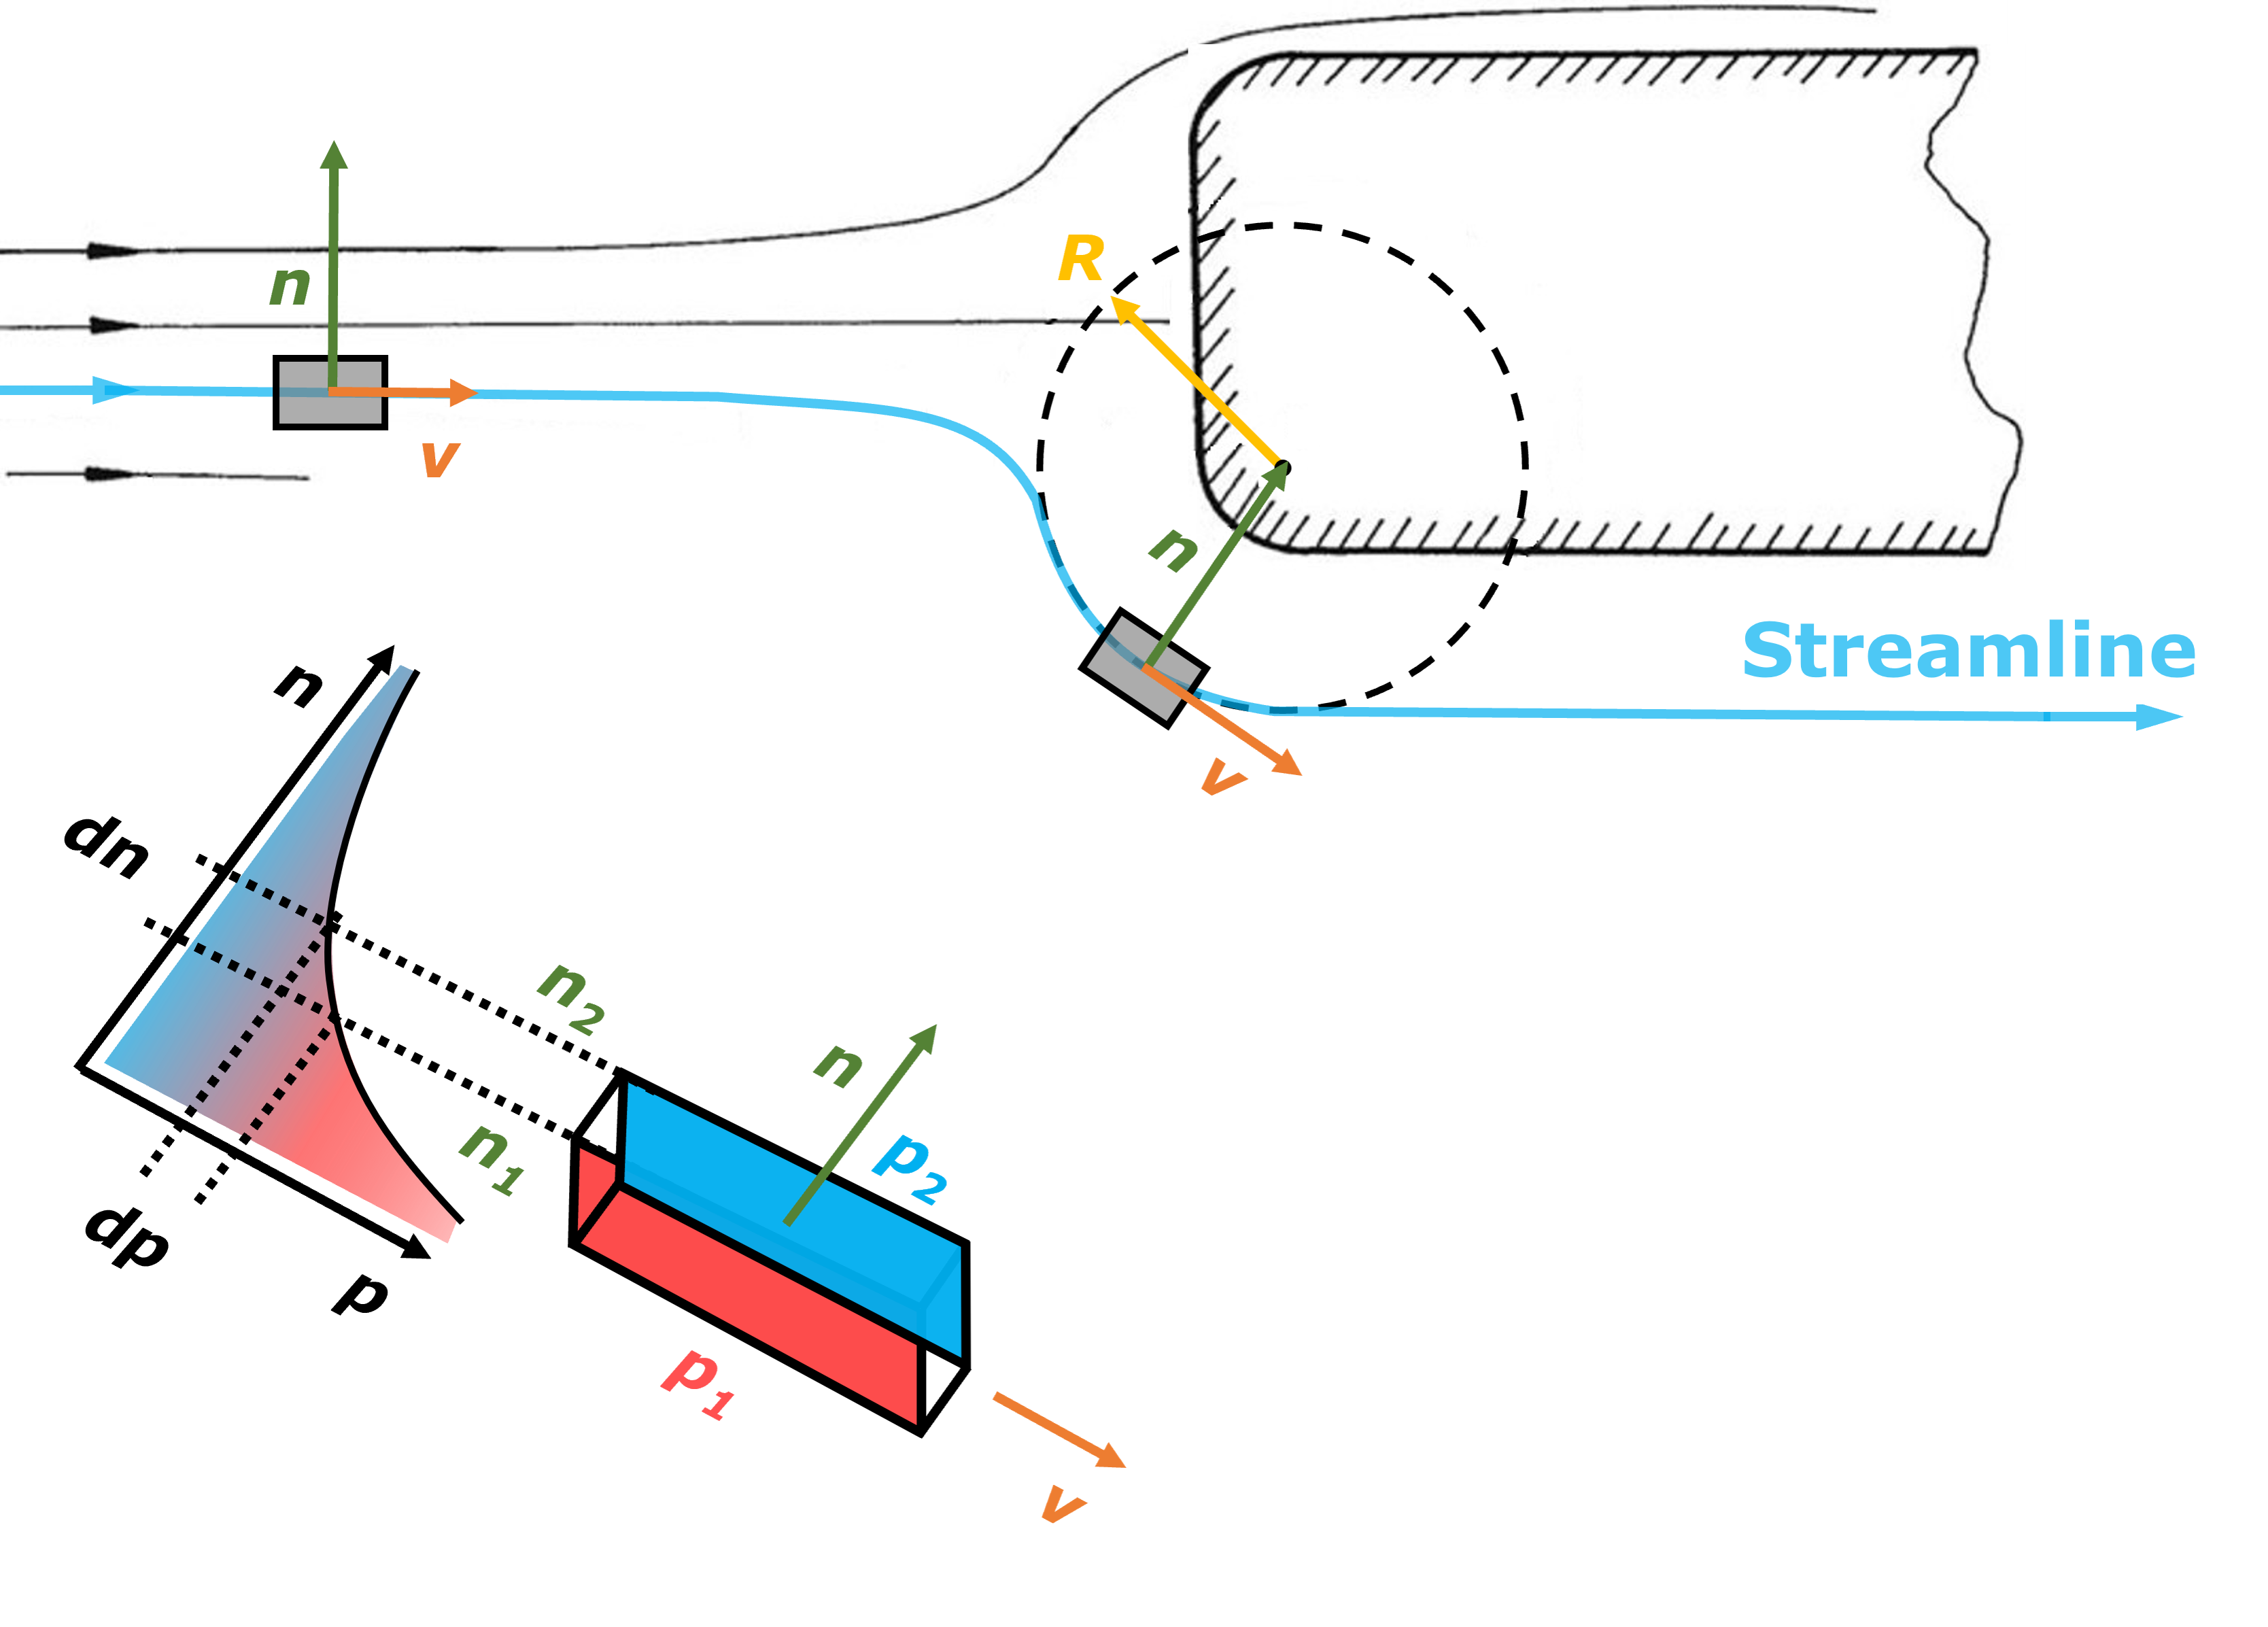
\includegraphics[width=\textwidth]{media/pressure_curvatur.png}
    \vspace*{-0.6cm}
    \begin{equation}
        \dfrac{dp}{dn} = -\rho\cdot\dfrac{v^2}{R}
    \end{equation}
\end{examplebox}

\vfill
\phantom{}
\end{multicols}

\newpage
\begin{multicols}{2}
\setlength{\columnsep}{1pt}

\section{Mass conservation}
\subsection{Continuity equation / Mass conservation}
\begin{theorybox}{Continuity equation}
    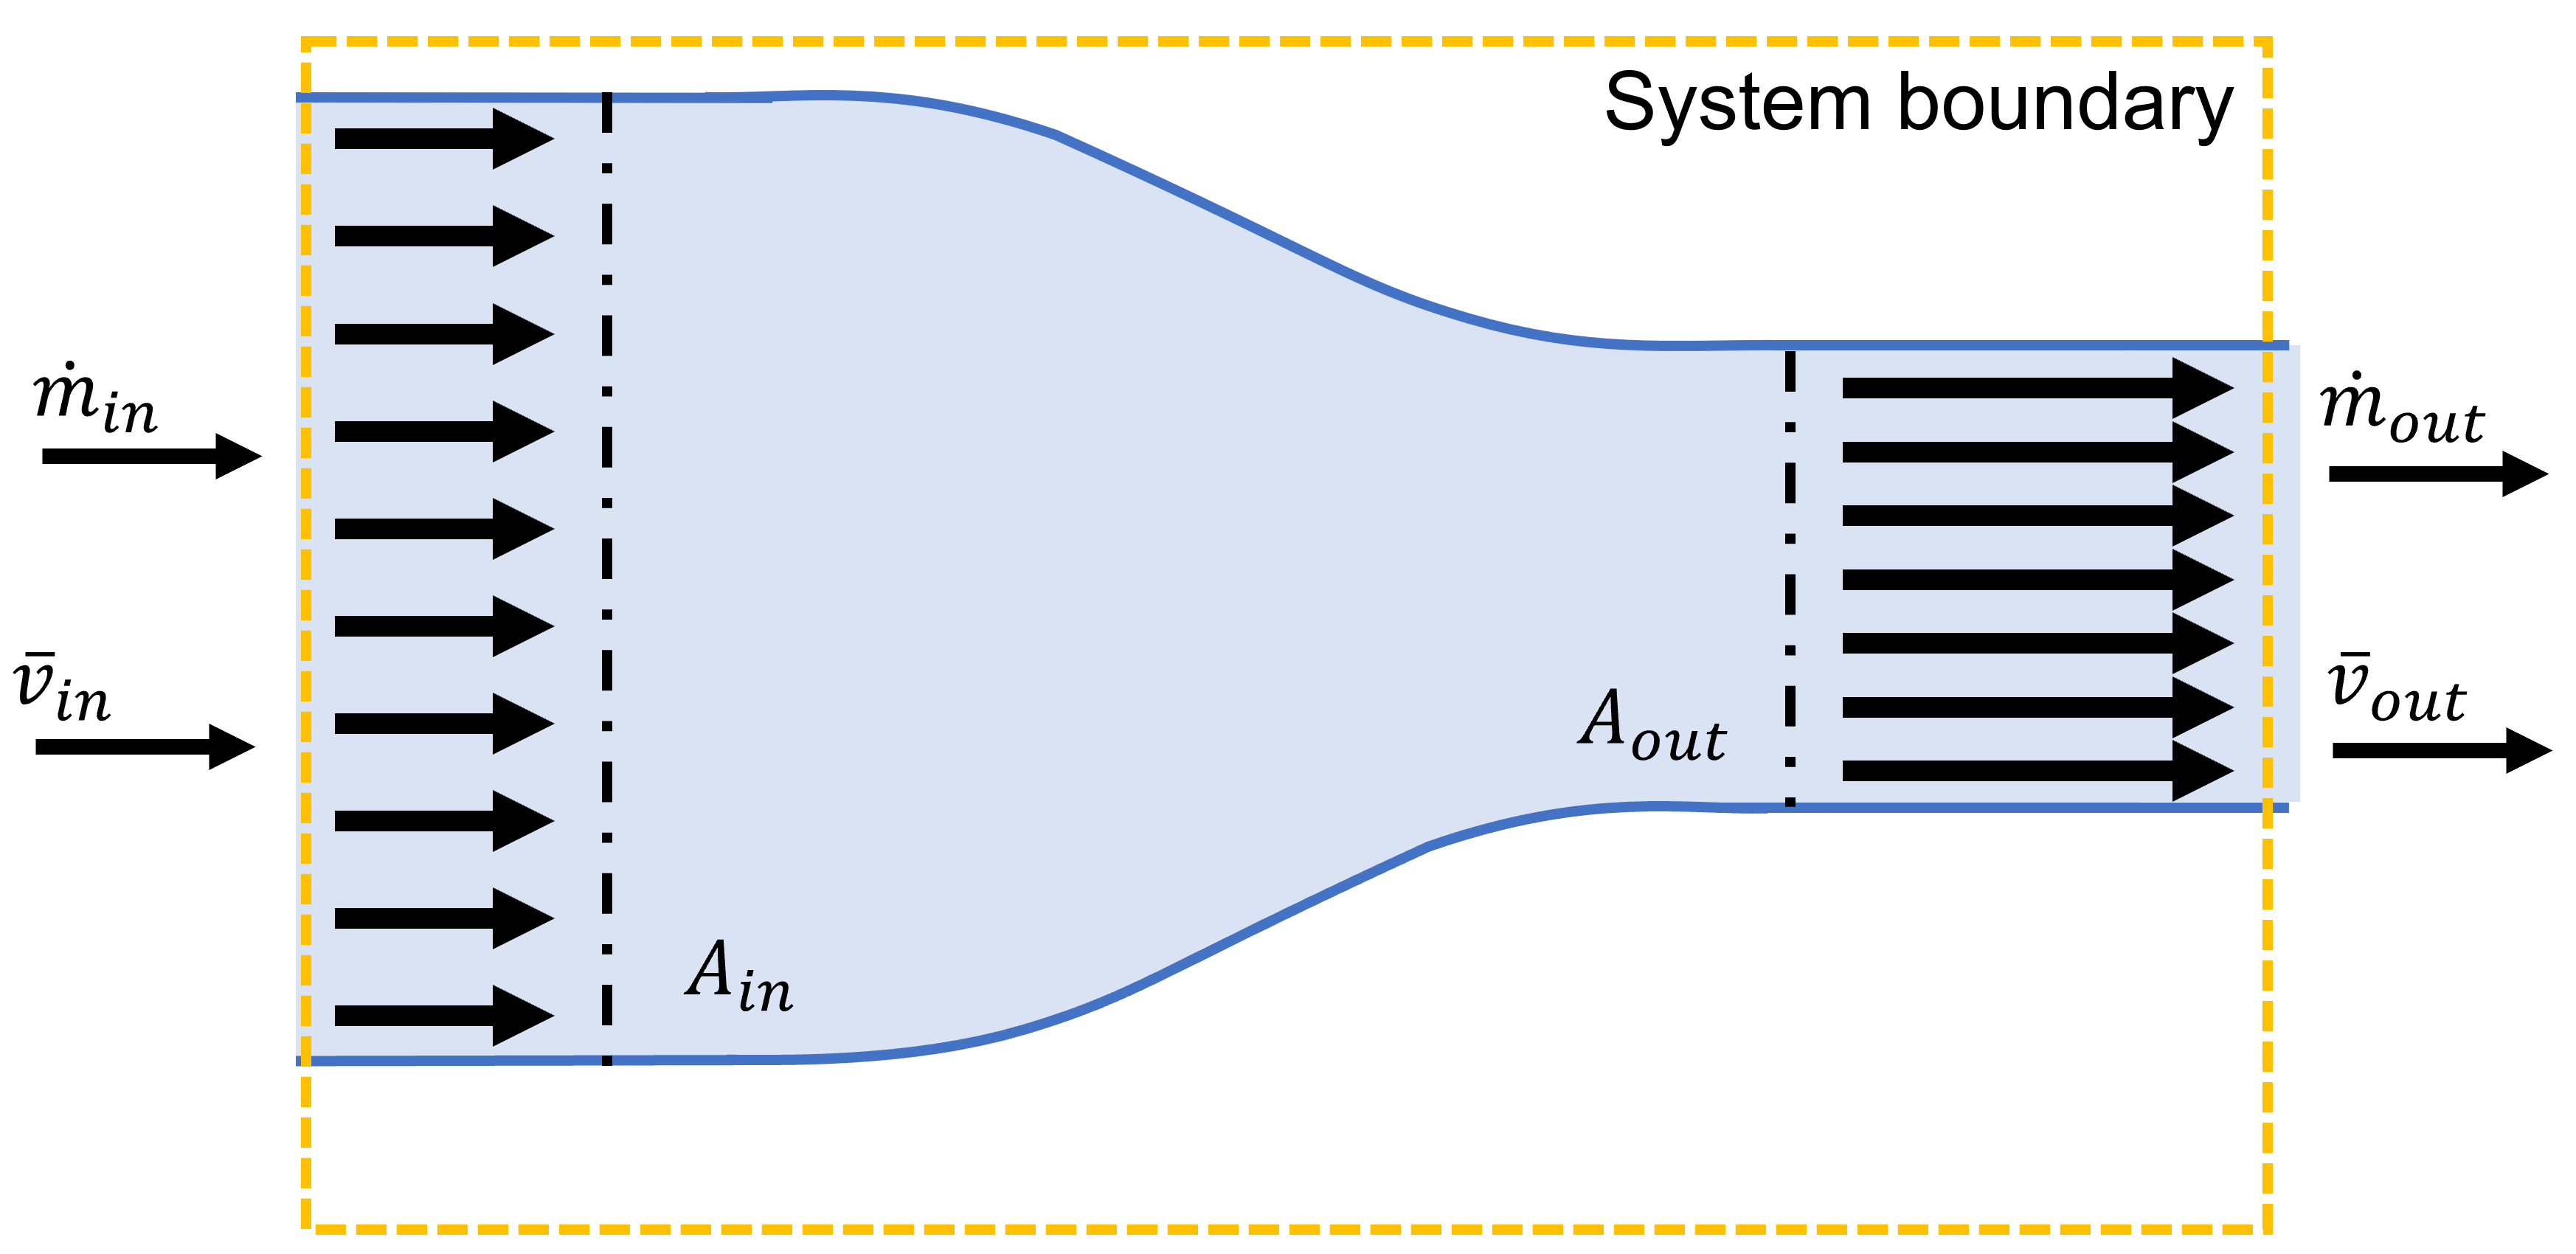
\includegraphics[width=\textwidth]{media/ContinuityBild1.png}
    \subsubsection{Steady mass-flow}
    \begin{equation}
    \dot m_{\rm in} = \dot m_{\rm out}
    \end{equation}

    \subsubsection{Incompressible fluid}
    \begin{equation}
    \dot m = \rho\,\dot V
    \quad\Longrightarrow\quad
    \dot V_{\rm in} = \dot V_{\rm out}
    \end{equation}

    \subsubsection{Streamline theory}
    \begin{equation}
    \dot V = \bar v\,A
    \quad\Longrightarrow\quad
    \bar v_{\rm in}\,A_{\rm in} = \bar v_{\rm out}\,A_{\rm out}
    \end{equation}
\end{theorybox}

\section{Energy conservation}
\subsection{Fluid mechanical energy conservation}
\begin{theorybox}{Derivation of the Bernoulli equation}
\vspace*{-0.3cm}
    \begin{equation}
        \dot{m}_1 \left(\dfrac{p_1}{\rho} + \dfrac{v_1^2}{2} + gz_1\right) = \dot{m}_2 \left(\dfrac{p_2}{\rho} + \dfrac{v_2^2}{2} + gz_2\right)
    \end{equation}

    This derivation is based on the assumption that the system has:
    
    \begin{minipage}[t]{0.48\linewidth}
        \begin{itemize}
            \item steady flow
            \item ideal fluid
            \item adiabatic process
        \end{itemize}
    \end{minipage}
    \hfill
    \begin{minipage}[t]{0.48\linewidth}
        \begin{itemize}
            \item no work in or out of the system
            \item 1D streamline flow
        \end{itemize}
    \end{minipage}
\subsubsection{Energy flow}
\vspace*{-0.5cm}
    \begin{align}
        \frac{dE}{dt} =\ 
        &\underbrace{\sum P + \sum \dot{Q}}_{
            \substack{
                \text{Energy flow} \\ \text{across system boundary}
            }
        } \notag \\
        &+ \underbrace{\sum_{in} \left[\dot{m}^{\swarrow} \cdot \left(h^{\swarrow} + \frac{v^{2\swarrow}}{2} + g z^{\swarrow}\right)\right]}_{
            \substack{
                \text{Energy transfer} \\ \text{mass in}
            }
        } \notag \\
        &- \underbrace{\sum_{out} \left[\dot{m}^{\nearrow} \cdot \left(h^{\nearrow} + \frac{v^{2\nearrow}}{2} + g z^{\nearrow}\right)\right]}_{
            \substack{
                \text{Energy transfer} \\ \text{mass out}
            }
        }
    \end{align}

    \vspace*{-0.5cm}
    \subsubsection{Outflow formula according to Torricelli}
    \begin{equation}
        gz_1 = \frac{v_2^2}{2} \Longrightarrow v_2 = \sqrt{2g\Delta z}
    \end{equation}
\end{theorybox}

\columnbreak

\subsection{Bernoulli equation}
\begin{formula}{Specific energy equation}
    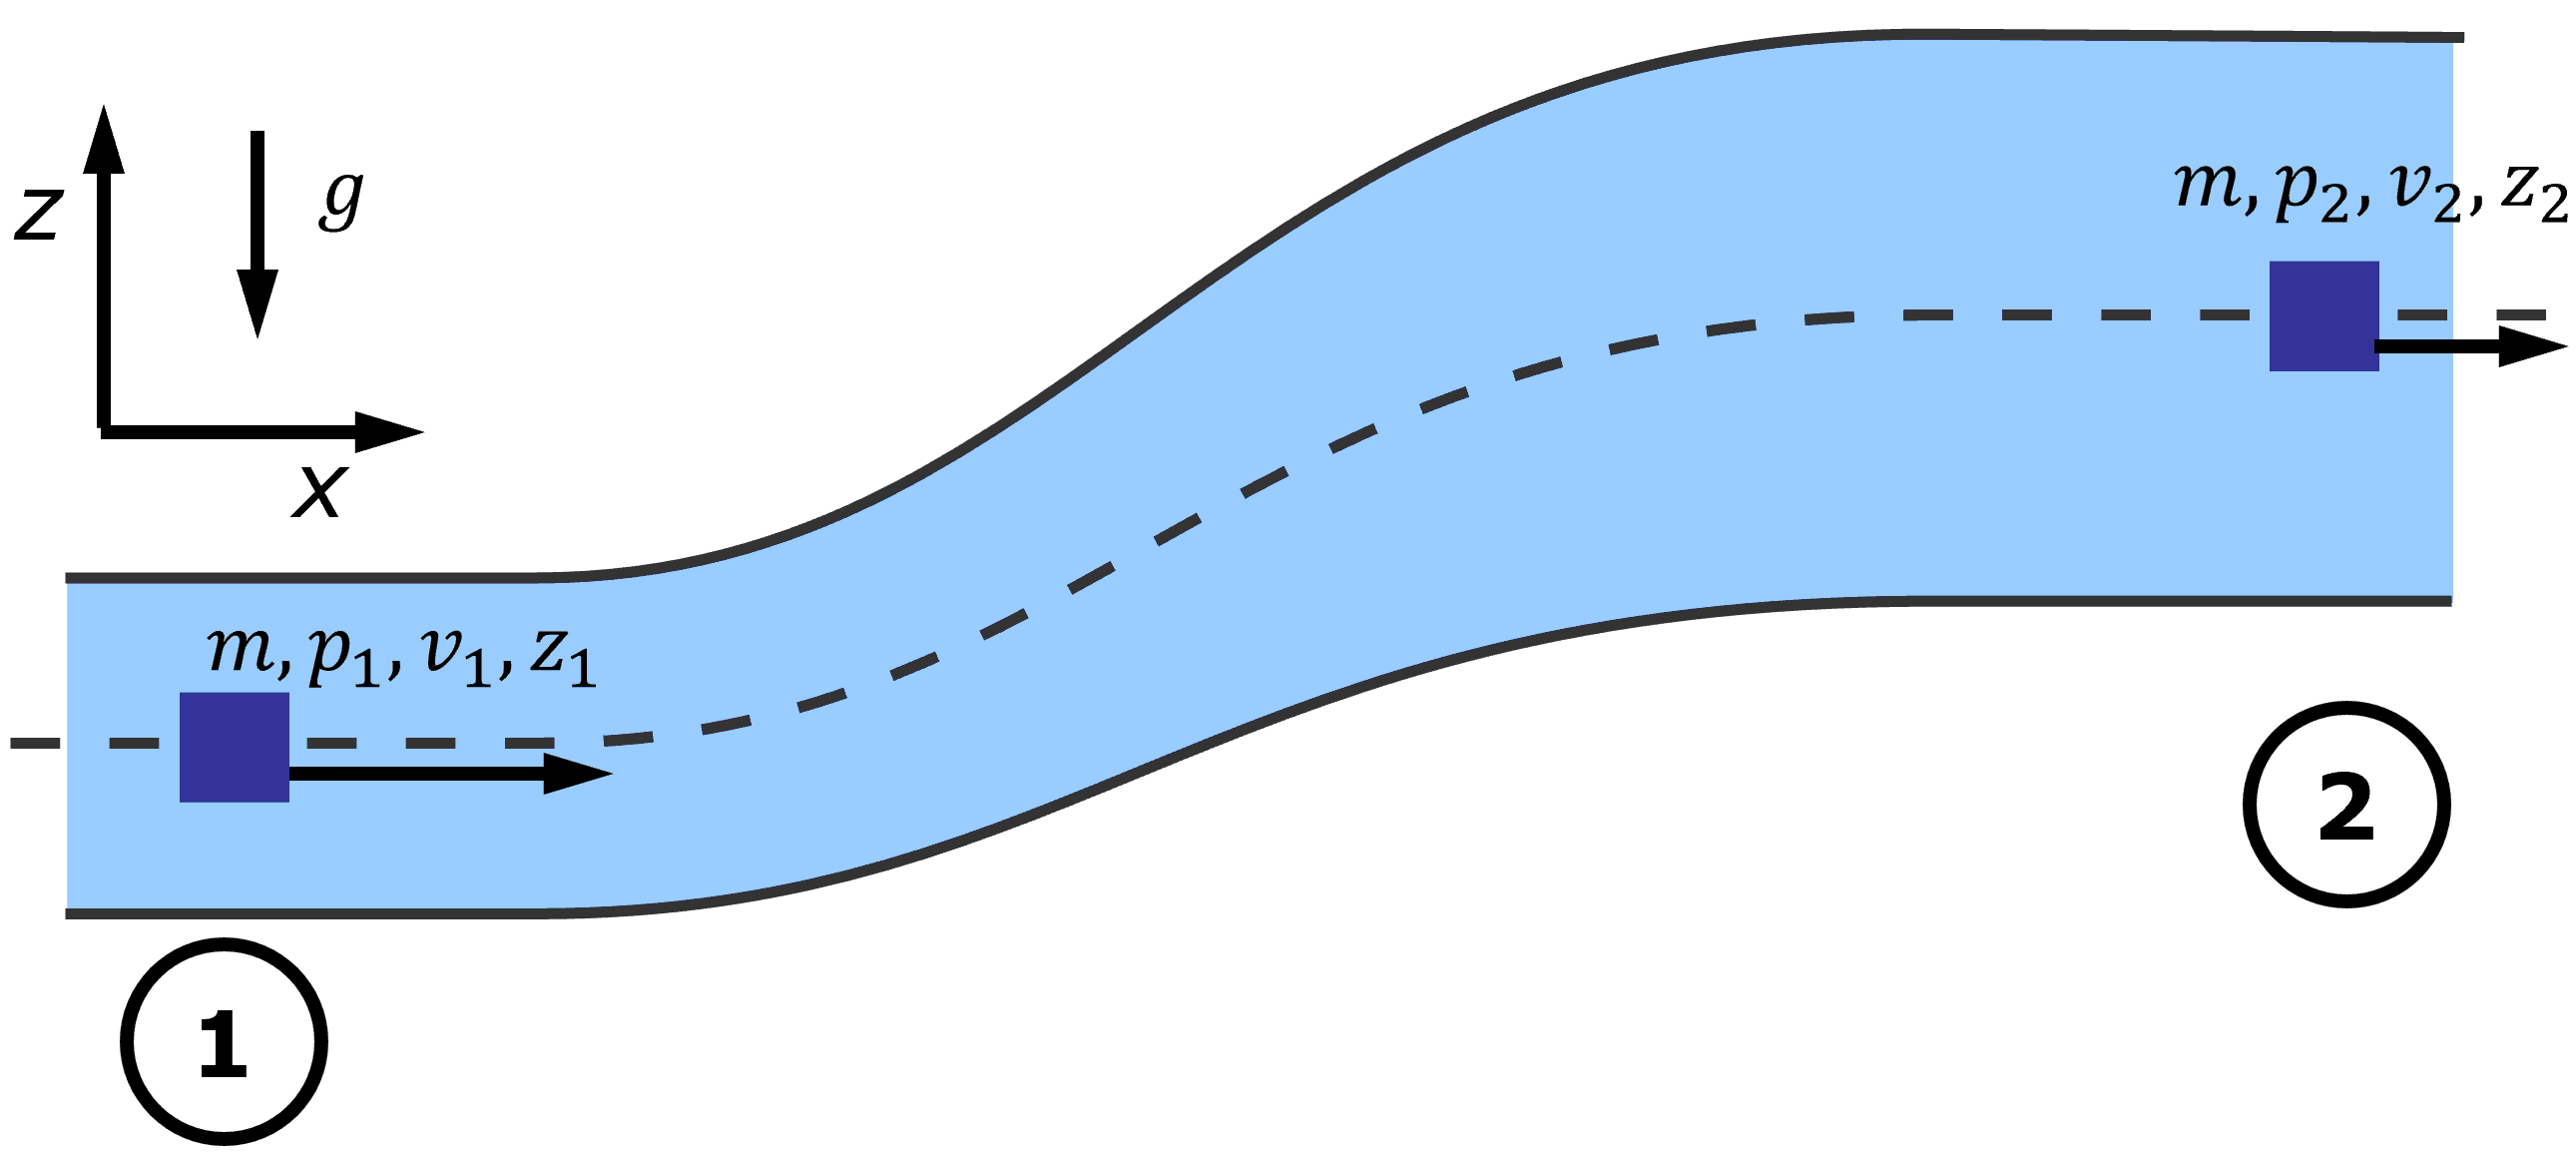
\includegraphics[width=\textwidth]{media/Bernoulli.png}
    \vspace*{-0.3cm}
    \begin{equation}
        \dfrac{p_1}{\rho} + \dfrac{v_1^2}{2} + gz_1 = \dfrac{p_2}{\rho} + \dfrac{v_2^2}{2} + gz_2 = {\rm const.} \left[\dfrac{J}{kg}\right]
    \end{equation}

    \subsubsection{Alternative forms}
    \textbf{Pressure equation}
    \begin{equation}
        p_1 + \dfrac{\rho v_1^2}{2} + \rho g z_1 = p_2 + \dfrac{\rho v_2^2}{2} + \rho g z_2 = {\rm const.} \left[Pa\right]
    \end{equation}

    \textbf{Height equation}
    \begin{equation}
        \dfrac{p_1}{\rho g} + \dfrac{v_1^2}{2g} + z_1 = \dfrac{p_2}{\rho g} + \dfrac{v_2^2}{2g} + z_2 = {\rm const.} \left[m\right]
    \end{equation}
\end{formula}

\begin{theorybox}{True energy equation}
    The Bernoulli equation states that the sum of these energies is constant along a streamline.
    \subsubsection{Pressure energy}
    \begin{equation}
        E_p = m\cdot \frac{p}{\rho} \left[J\right]
    \end{equation}

    \subsubsection{Kinetic energy}
    \begin{equation}
        E_{\rm kin} = m\cdot \frac{v^2}{2} \left[J\right]
    \end{equation}

    \subsubsection{Potential energy}
    \begin{equation}
        E_{\rm pot} = m\cdot g\cdot z \left[J\right]
    \end{equation}

\subsubsection{Energy conservation}
\vspace*{-0.5cm}
\begin{align}
    E_{p,1} + E_{\rm kin,1} + E_{\rm pot,1} &= E_{p,2} + E_{\rm kin,2} + E_{\rm pot,2} \notag \\[1.5ex]
    m\left(\dfrac{p_1}{\rho}+\dfrac{v_1^2}{2}+gz_1\right) &= m\left(\dfrac{p_2}{\rho}+\dfrac{v_2^2}{2}+gz_2\right)
\end{align}
\end{theorybox}

\subsection{Hydrostatics}
\begin{formula}{Fundamental law of hydrostatics}
    \begin{equation}
        p = p_0 + \rho g h = {\rm const.} \left[\rm Pa\right]
    \end{equation}
    derived from:
    \begin{equation}
        p = p_0 + \dfrac{F_g}{A} = p_0 + \dfrac{mg}{A} = p_0 + \dfrac{\rho hAg}{A}
    \end{equation}
\end{formula}

\vfill
\phantom{}
\end{multicols}

\newpage
\begin{multicols}{2}
\setlength{\columnsep}{1pt}

\subsection{Venturi effect experiment}
\begin{examplebox}{Venturi effect}
    \textbf{Height -- pressure difference at $\dot{V} = 6$ l/s}\\[1ex]
    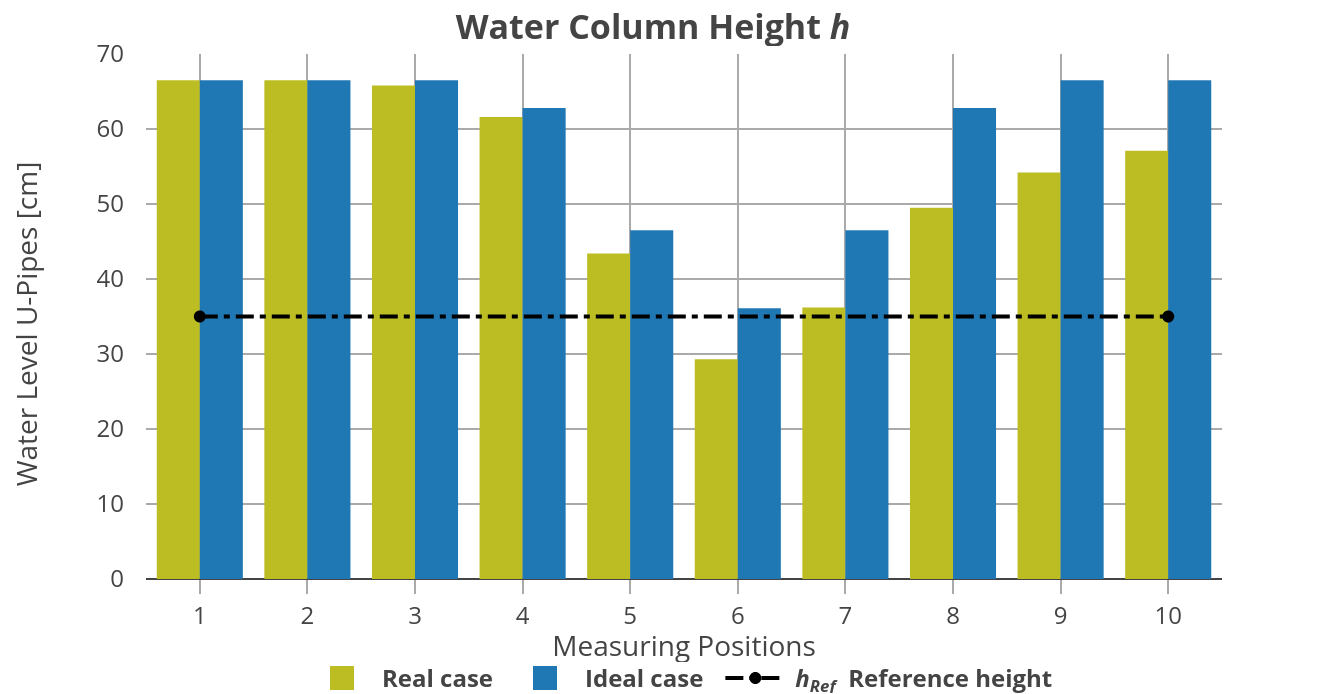
\includegraphics[width=\textwidth]{media/venturi.png}

    \begin{formula}{Relative static pressure $p_{\rm rel}$}
        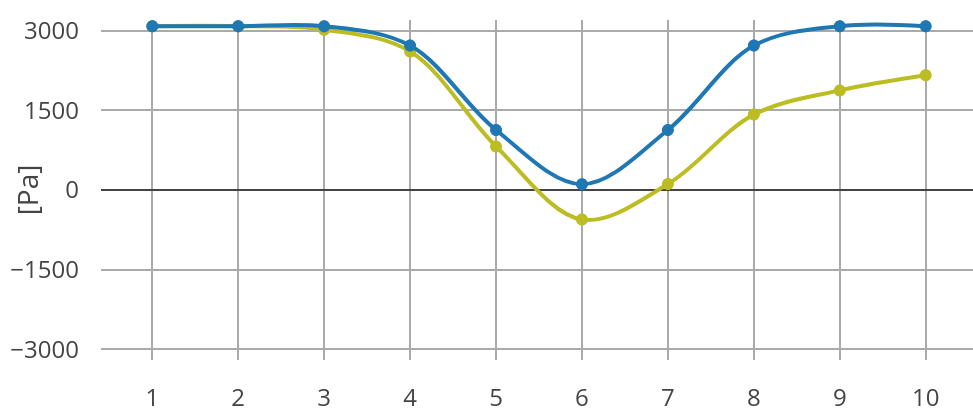
\includegraphics[width=\textwidth]{media/venturi_relative.png}
        \vspace*{-0.3cm}
        \begin{equation}
            p_{\rm rel} = p_{\rm hydro} = \rho g \left(h-h_{\rm ref}\right)
        \end{equation}
    \end{formula}
    \begin{formula}{Dynamic pressure $p_{\rm dyn}$}
        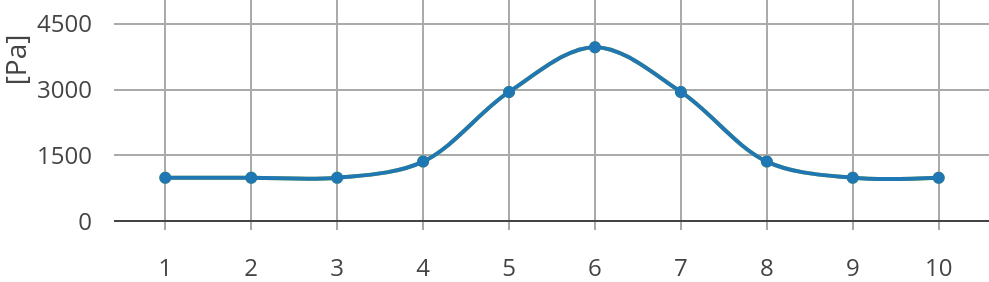
\includegraphics[width=\textwidth]{media/venturi_dyn.png}
        \vspace*{-0.3cm}
        \begin{equation}
            p_{\rm dyn} = \rho\dfrac{v^2}{2}
        \end{equation}
    \end{formula}
    \begin{formula}{Dynamic pressure $v$}
        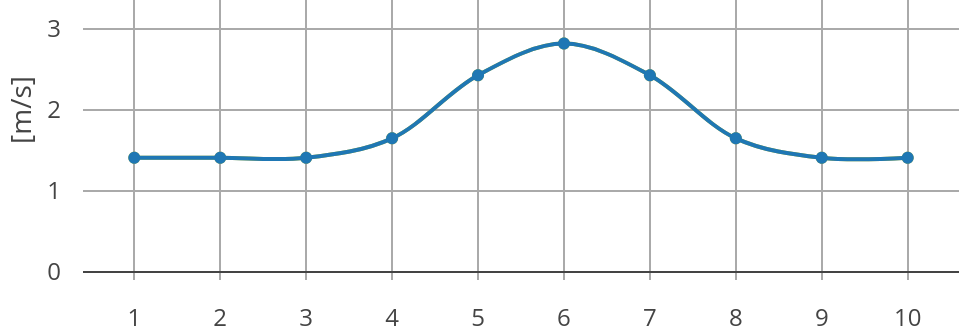
\includegraphics[width=\textwidth]{media/venturi_velocity.png}
        \vspace*{-0.3cm}
        \begin{equation}
            v=\dfrac{\dot{V}}{A}
        \end{equation}
    \end{formula}
    \begin{formula}{Pressure difference $\Delta p$}
        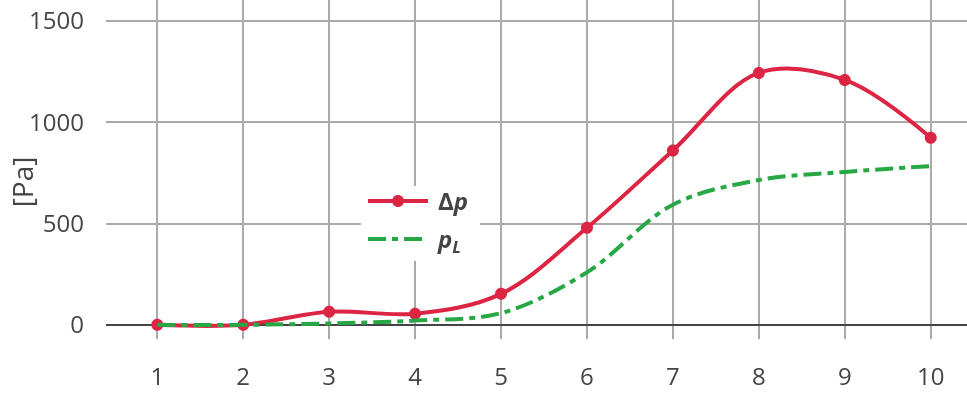
\includegraphics[width=\textwidth]{media/venturi_pressure.png}
        \vspace*{-0.3cm}
        \begin{equation}
           \Delta p = p_{\rm NoFric} - p_{\rm real} \Longrightarrow p_V \sim v^2
        \end{equation}
    \end{formula}
\end{examplebox}

\vfill
\columnbreak
\begin{examplebox}{Venturi effect}
    \textbf{Measurament points}\\[1ex]
    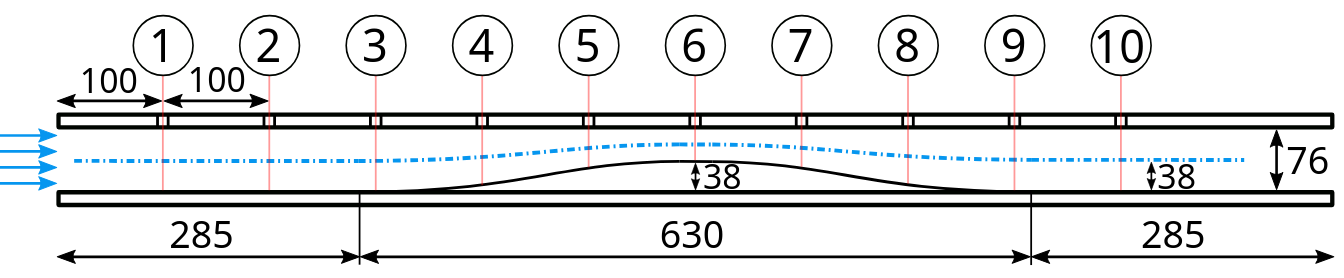
\includegraphics[width=\textwidth]{media/venturi_points.png}

    \textbf{Measurament shear flow}\\[1ex]
    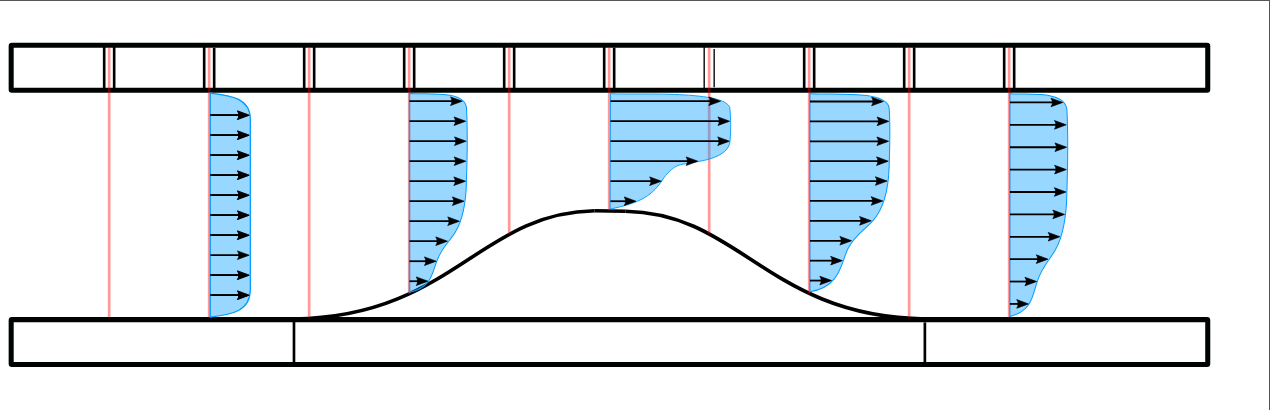
\includegraphics[width=\textwidth]{media/venturi_flow.png}
\end{examplebox}

\subsection{Contraction coefficient}
\begin{theorybox}{Outflow contraction coefficient $\alpha$}
    \begin{center}
        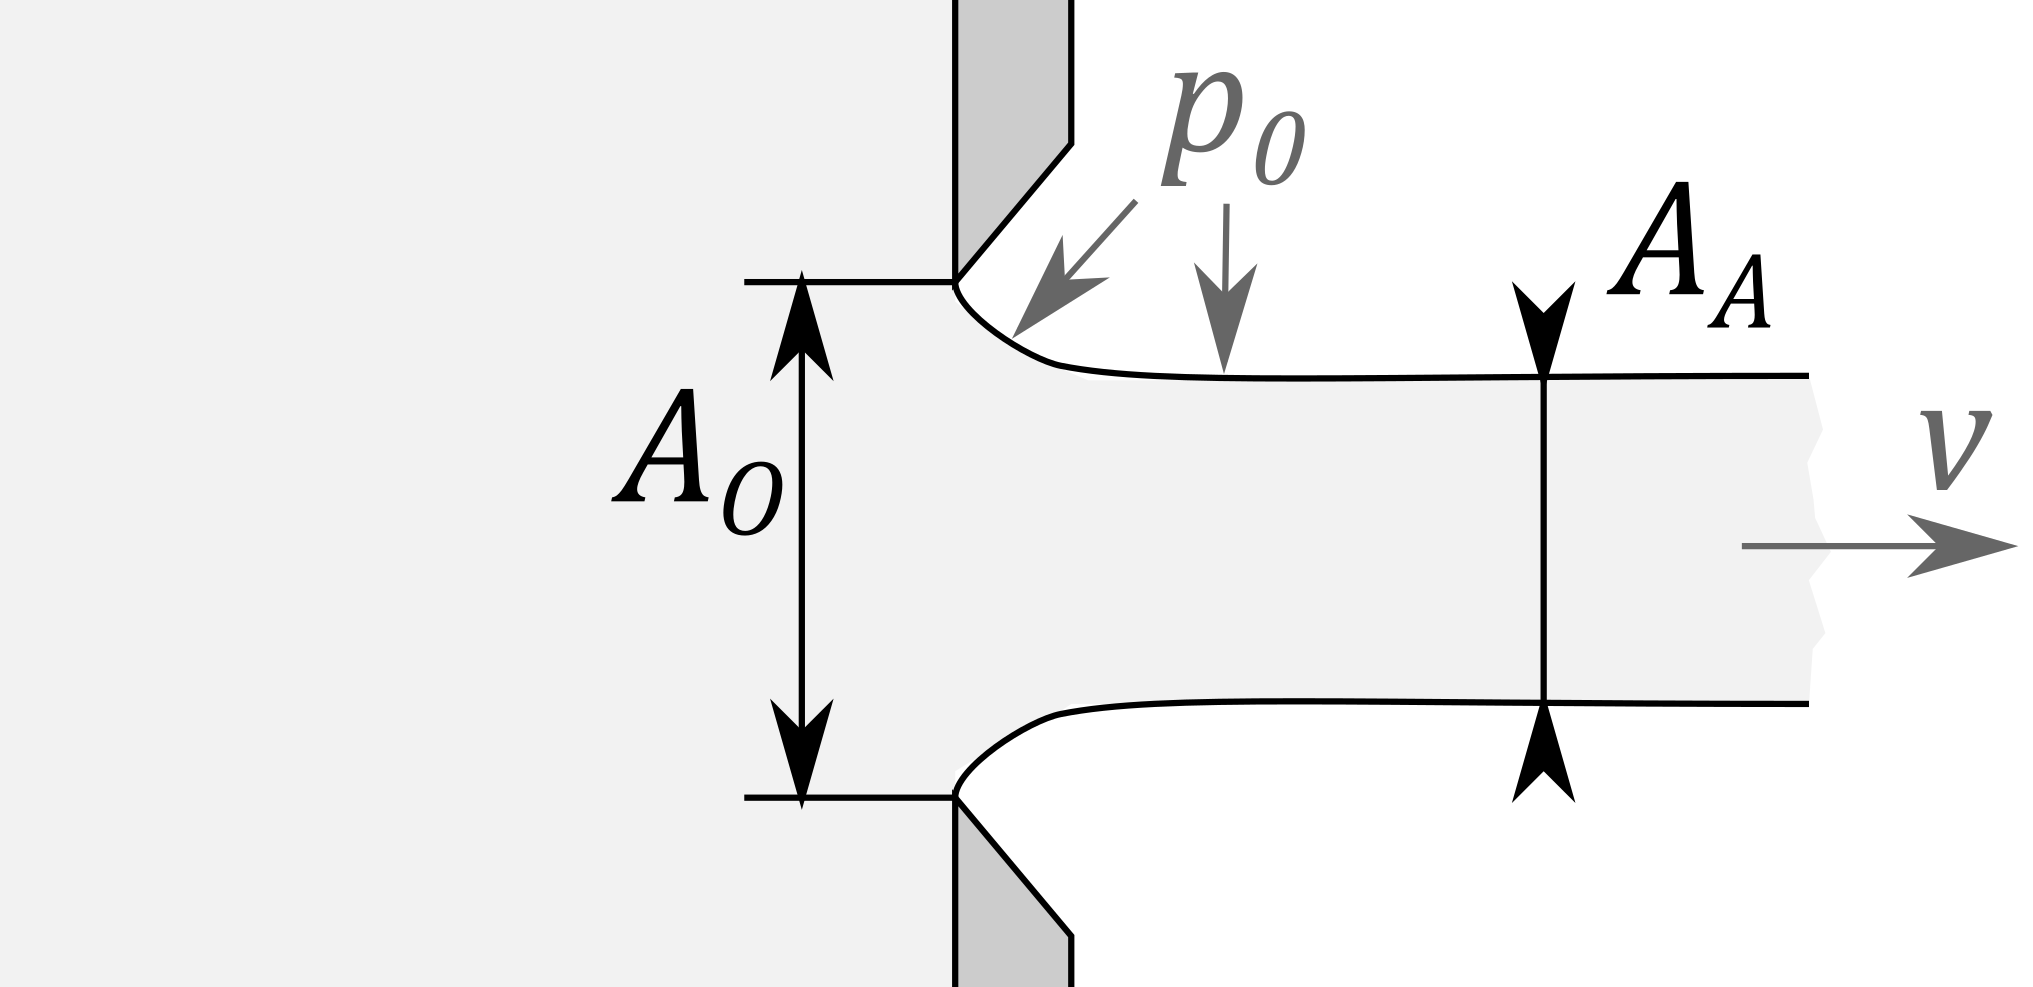
\includegraphics[width=.75\textwidth]{media/contraction.png}
    \end{center}
    \begin{equation}
        \alpha = \dfrac{A_{\rm actual}}{A_{\rm opening}} = \dfrac{\pi}{2 + \pi} \approx 0.611 [-]
    \end{equation}
\end{theorybox}

\subsection{Energy line diagram}
\begin{theorybox}{Ideal fluid energy line diagram}
    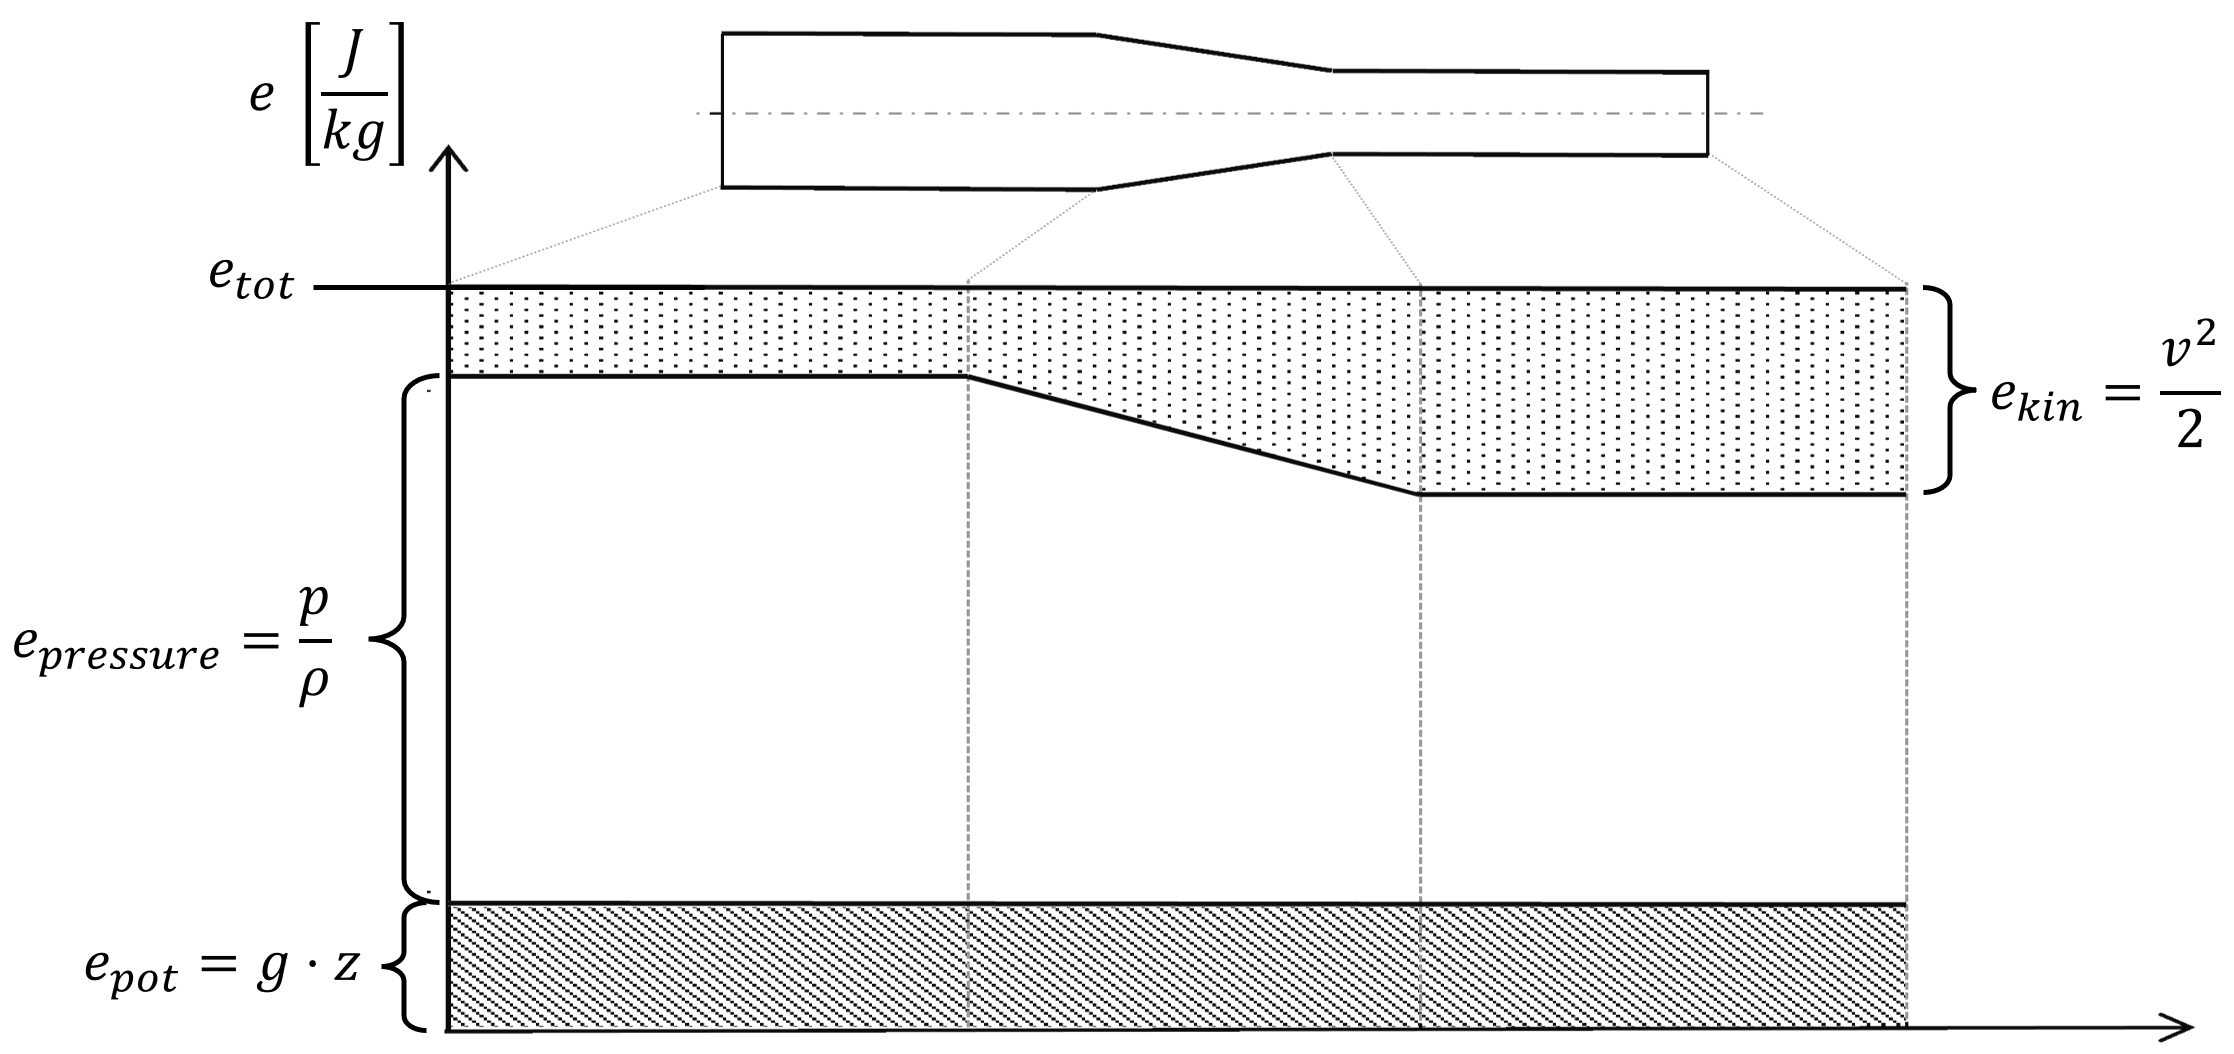
\includegraphics[width=\textwidth]{media/EGL_Duese_EN.PNG}
\end{theorybox}

\begin{theorybox}{Extended energy line diagram}
    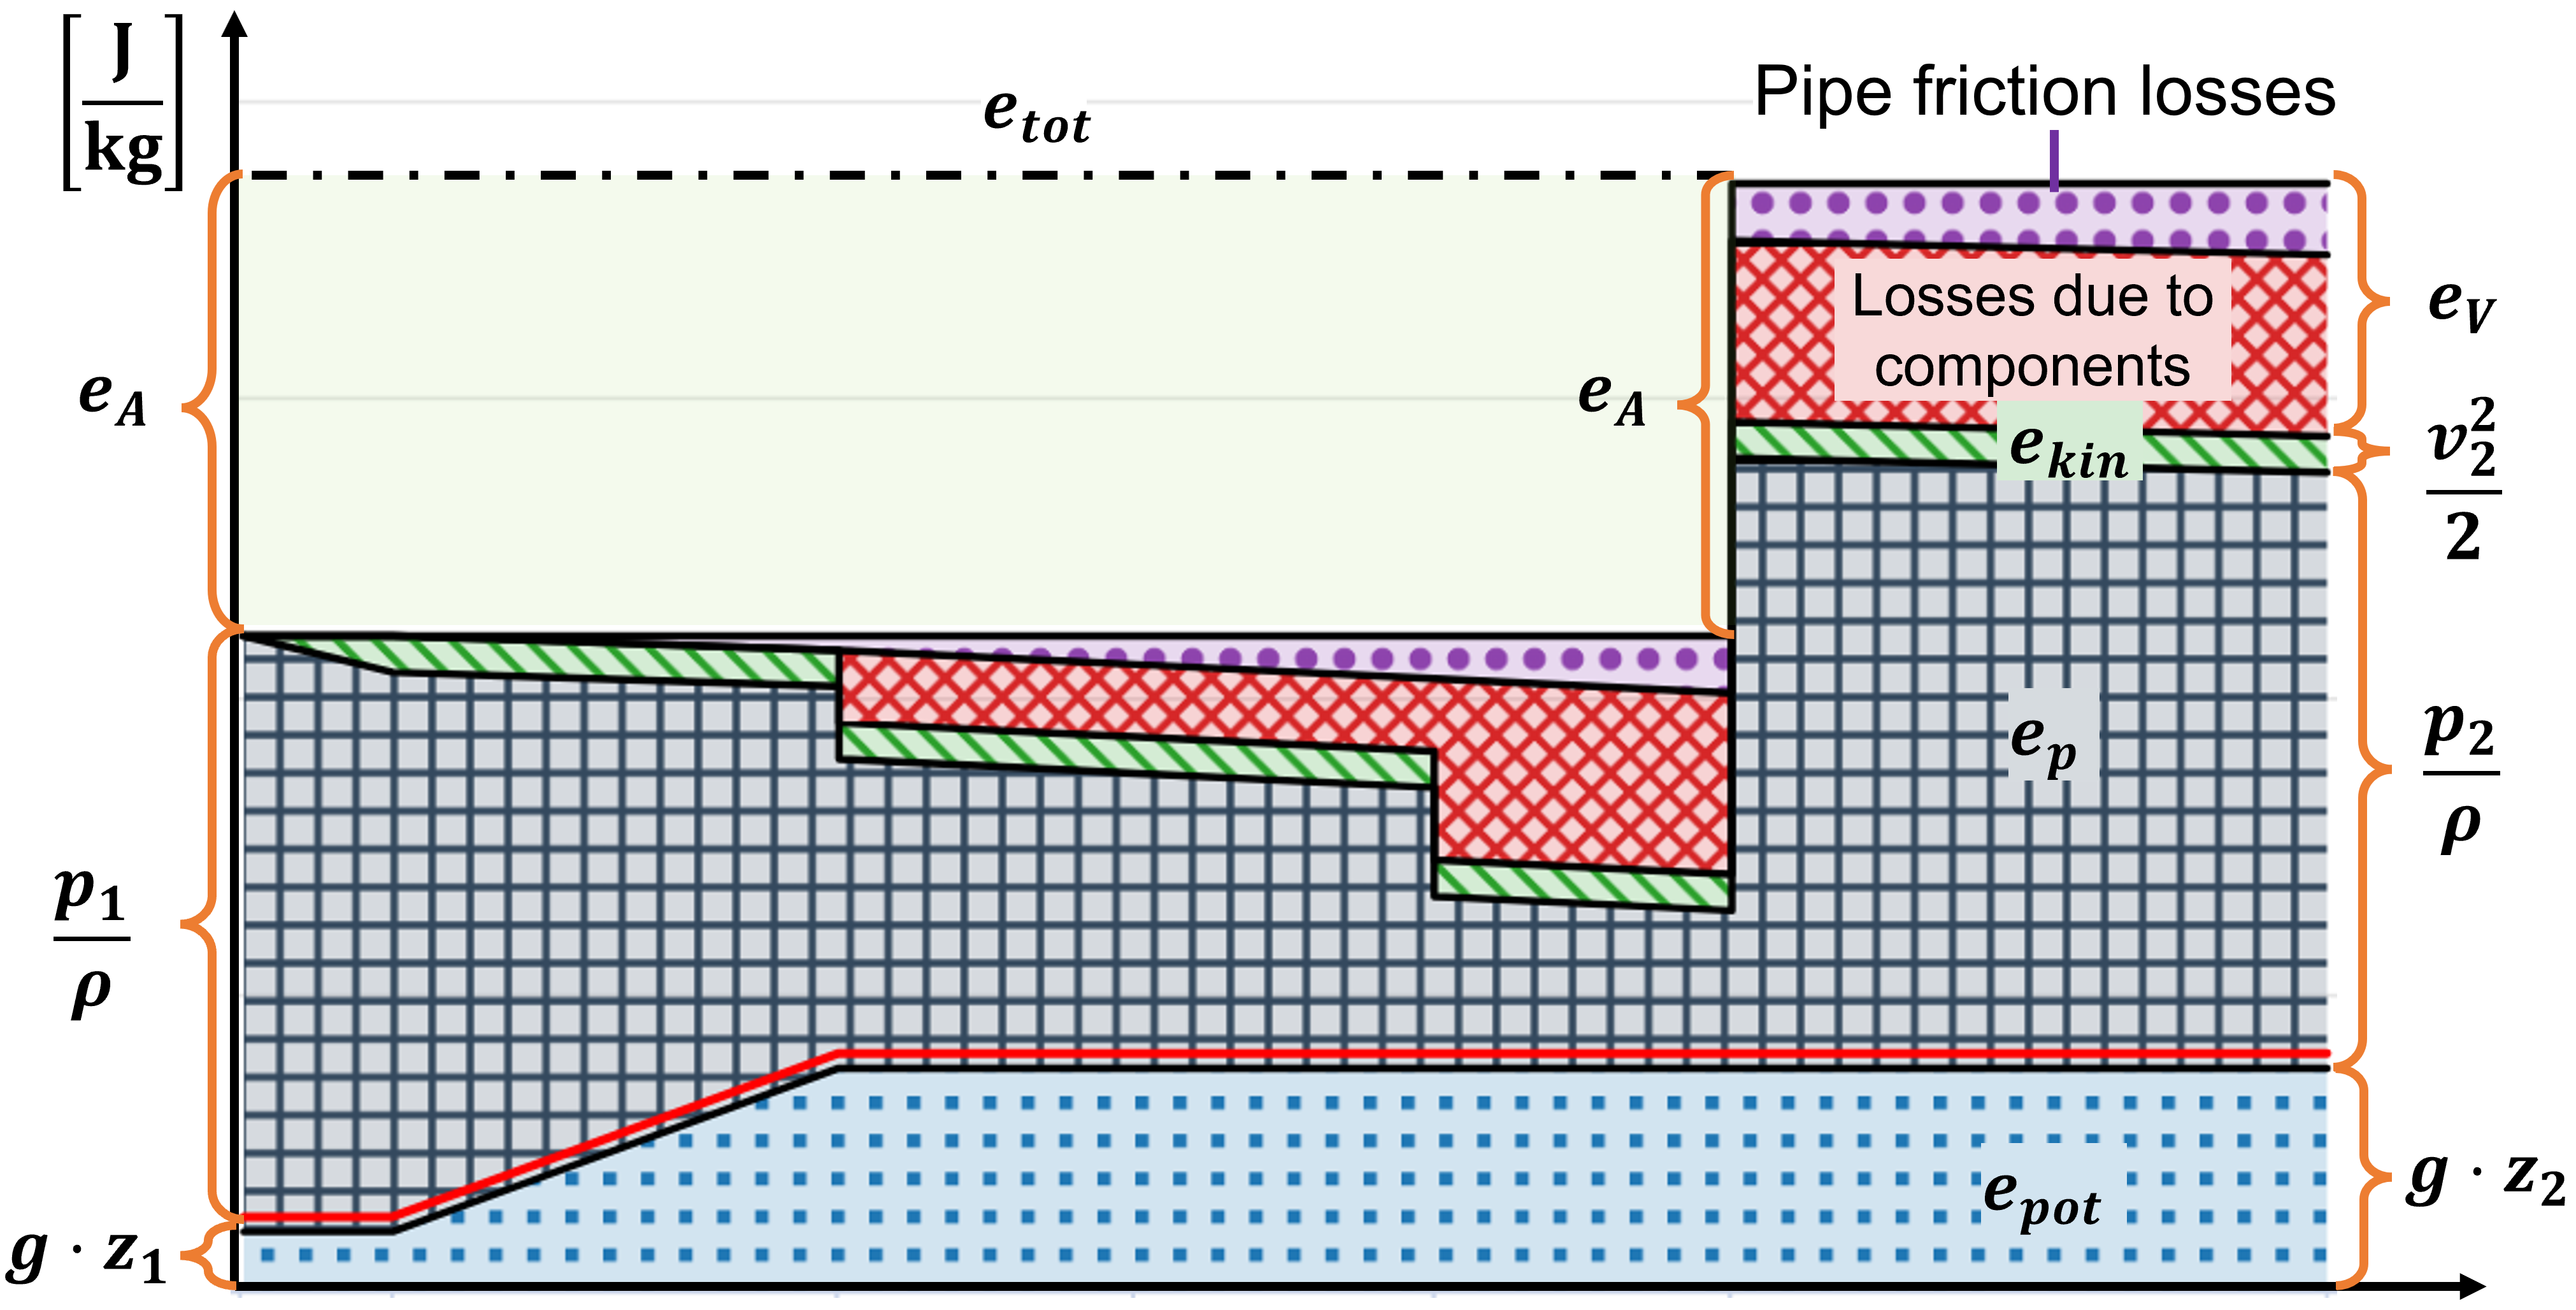
\includegraphics[width=\textwidth]{media/04_energyLineDiagram_vGB.png}
\end{theorybox}

\vfill
\end{multicols}

\newpage
\begin{multicols}{2}
\setlength{\columnsep}{1pt}

\subsection{Extended Bernoulli equation}
\begin{formula}{Extension of the Bernoulli equation}
    \vspace*{-0.4cm}
    \begin{align}
        &\dfrac{p_1}{\rho} + \dfrac{v_1^2}{2} + gz_1 + e_A = \dfrac{p_2}{\rho} + \dfrac{v_2^2}{2} + gz_2 + e_V \left[\frac{J}{kg}\right] \notag \\
        &E_{p,1} + K_1 + U_1 + E_A = E_{p,2} + K_2 + U_2 + E_V \left[J\right]
    \end{align}
\end{formula}

\subsubsection{Additional terms}
\begin{theorybox}{Work term $e_A$}
    \begin{equation}
        e_A = \frac{p_A}{\rho} = gz_A = \frac{E_A}{m} = \frac{P_A}{\dot{m}} \left[\frac{J}{kg}\right]
    \end{equation}
    where:\\
    \begin{minipage}[t]{0.48\linewidth}
        $e_A$: work term [J/kg] \\
        $p_A$: pressure diff [Pa] \\
        $z_A$: height difference [m]
    \end{minipage}
    \hfill
    \begin{minipage}[t]{0.48\linewidth}
        $E_A$: energy difference [J] \\
        $P_A$: power difference [W]
    \end{minipage}\\[1.5ex]

    If energy is added to the fluid along a streamline from point 1 to point 2
    (eg. a pump), the total energy at point 2 becomes higher than at point 1.\\

    \textbf{Sign convention}\\
    $\mathbf{e_A > 0}$: work is done on the fluid\\
    \textrightarrow\ energy is added to the fluid (eg. pump);\\

    $\mathbf{e_A < 0}$: work is done by the fluid\\
    \textrightarrow\ energy is extracted from the fluid (eg. turbine).

    \begin{formula}{Pump and turbine work $Y$}
        In the pressure equation, the pressure $p_A$ increase (or decrease with a turbine) can
        be read directly at the working term, hence:
        \begin{equation}
            e_w = Y = \frac{W_A}{\dot{m}} = \frac{E_A}{m} = H\cdot g = \frac{p_A}{\rho} \left[\frac{J}{kg}\right]
        \end{equation}

        The hydraulic power $P_{\rm hyd}$ is then given by:
        \begin{equation}
            P_{\rm hyd} = \dot{m}\cdot Y = \dot{V}\cdot \rho\cdot Y = \rho\cdot \dot{V} \cdot g \cdot H \left[W\right]
        \end{equation}
    \end{formula}
\end{theorybox}

\begin{theorybox}{Specific loss term $e_V$}
    \begin{equation}
        e_V = \frac{p_V}{\rho} = gz_V = \frac{E_V}{m} = \frac{P_V}{\dot{m}} \left[\frac{J}{kg}\right]
    \end{equation}
    where:\\
    \begin{minipage}[t]{0.48\linewidth}
        $e_V$: loss term [J/kg] \\
        $p_V$: pressure diff [Pa] \\
        $z_V$: height loss [m]
    \end{minipage}
    \hfill
    \begin{minipage}[t]{0.48\linewidth}
        $E_V$: energy loss [J] \\
        $P_V$: power loss [W]
    \end{minipage}\\[1.5ex]

    The effects of a viscous fluid along a stramline from point 1 to point 2 are taken into
    account by $e_V$.

    \begin{formula}{Pressure loss $\Delta p_V$}
        \vspace*{-0.48cm}
        \begin{equation}
            \Delta p_V = e_V \cdot \rho = \frac{E_V\cdot \rho}{m} = g\cdot z_V \cdot \rho = \zeta\cdot \rho \cdot \frac{v^2}{2} \left[Pa\right]
        \end{equation}
    \end{formula}
\end{theorybox}

\vfill
\columnbreak

\subsection{Loss behavior in turbolent flows}
\begin{formula}{Zeta value}
    \begin{equation}
        \zeta = \frac{2\cdot \Delta p_V}{\rho\cdot v^2}
    \end{equation}
\end{formula}

\begin{theorybox}{Total pressure loss}
    If multiple losses occur in a system due to sequentially connected hydraulic components,
    the ttal loss $\Delta p_{V,\rm tot}$ is given by the sum of the individual losses:
    \vspace*{-0.3cm}
    \begin{align}
        \Delta p_{V,\rm tot} &= \sum_{i} \Delta p_{V,i} = \sum_{i} \zeta_i\cdot \rho\cdot \frac{v^2_i}{2} \left[Pa\right]\\
        \Delta p_{V,\rm tot} &= \rho \cdot \frac{v^2}{2} \cdot \sum_{i} \zeta_i = \rho\cdot \frac{v^2}{2} \cdot \zeta_{\rm tot} \left[Pa\right]
    \end{align} 
\end{theorybox}

\begin{theorybox}{Pressure head (prevalenza)}
    The pressure head $H$ is the (energy) height corresponding to its
    specific potential energy $e_A$:
    \begin{equation}
        H = \frac{e_A}{g} = \frac{\Delta p_A}{\rho\cdot g} \left[m\right]
    \end{equation}
\end{theorybox}

\begin{examplebox}{U-Tube manometer}
    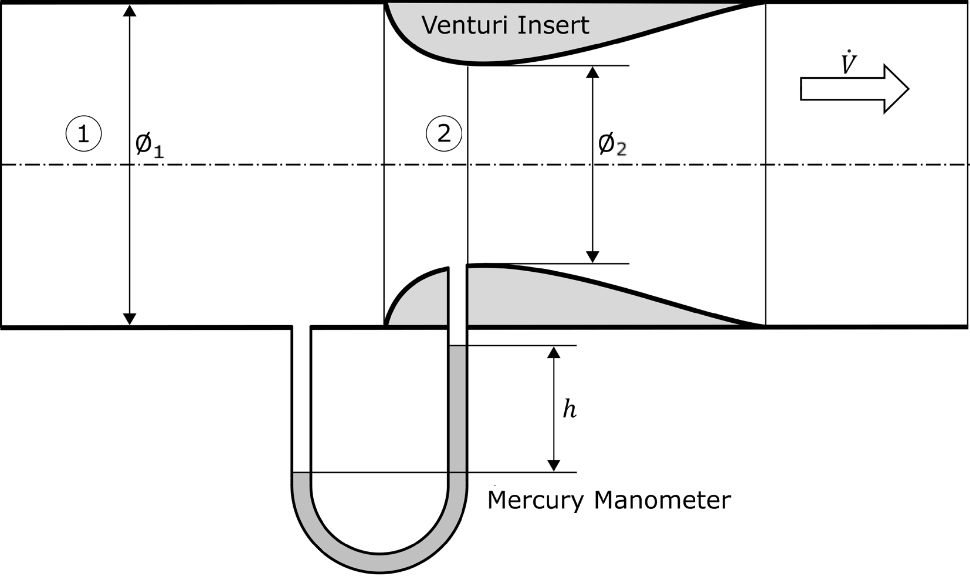
\includegraphics[width=\textwidth]{media/venturi_ex.png}
    \begin{equation}
        h = \frac{\rho \left(v_ 2^2 - v_1^2\right)}{2g\left(\rho_{\rm Hg} - \rho_w\right)}
    \end{equation}
\end{examplebox}

\subsection{Efficiency}
\begin{theorybox}{Efficiency factor $\eta$}
    \begin{align}
        \eta &= \frac{P_{\rm out}}{P_{\rm in}} = \frac{\rm Benefit}{\rm Effort}\\[2ex]
        \eta_{\rm hyd} &= \frac{P_{\rm real}}{P_{\rm ideal}} = \frac{\dot{m} \cdot e_{\rm real}}{\dot{m} \cdot e_{\rm ideal}} = \frac{e_A - e_V}{e_A} \notag\\
        \eta_{\rm hyd} &= \left(= \frac{\Delta e_k + \Delta e_{\rm pot} + \Delta e_p}{e_A}\right)
    \end{align}

    \subsubsection{Volumetric efficiency $\eta_{\rm vol}$}
    \begin{equation}
        \eta_{\rm vol} = \frac{\dot{m}_{\rm real}}{\dot{m}_{\rm ideal}} = \frac{\dot{V}_{\rm real}}{\dot{V}_{\rm ideal}}
    \end{equation}
\end{theorybox}

\vfill
\phantom{}
\end{multicols}

\newpage
\begin{multicols}{2}
\setlength{\columnsep}{1pt}

\begin{theorybox}{Efficiency factor $\eta$}
    \subsubsection{Efficiency of a pump-driven system}
    \begin{equation}
        \eta_{\rm pump} = \frac{P_{\rm hyd}}{P_{\rm mech}} = \frac{\dot{m} \cdot Y}{M\cdot \omega}
    \end{equation}
    
    \begin{equation}
        \eta_{\rm tot} = \underbrace{{\eta_{\rm el} \cdot \eta_{\rm mech} \cdot \eta_{\rm vol}}}_{\rm Pump} \cdot \eta_{\rm hyd}^{\rm system}
    \end{equation}

    In the case of an eletrically driven pump, the effective power transferred to the fluid is thus:
    \begin{equation}
        P_{\rm eff} = P_{\rm el} \cdot \eta_{\rm tot}
    \end{equation}

    \subsubsection{Efficiency of a turbine-driven system}
    \begin{equation}
        \eta_{\rm turbine} = \frac{P_{\rm mech}}{P_{\rm hyd}} = \eta_{\rm mech} \cdot \eta_{\rm hyd}
    \end{equation}
    
    \begin{equation}
        \eta_{\rm tot} = \eta_{\rm turbine} \cdot \eta_{\rm el} = \eta_{\rm mech} \cdot \eta_{\rm hyd} \cdot \eta_{\rm el}
    \end{equation}
\end{theorybox}

\section{Pipe flows}
\subsection{Flow characteristics}
\begin{formula}{Reynolds number in pipes}
    \begin{equation}
        Re = \frac{v_m \cdot d}{\nu}
    \end{equation}
\end{formula}

\begin{theorybox}{Pipe flows}
    \subsubsection{Laminar pipe flow}
    The pressure loss of a laminar pipe flow is described by the Hagen-Poiseuille:
    \begin{align}
        &v(r) = \frac{p_1 - p_2}{4\eta \cdot l}\left(R^2 - r^2\right)\\
        &v_m = \frac{v_{\rm max}}{2} = \frac{p_1 - p_2}{8\eta \cdot l}\cdot R^2 \notag \\
        &v_m = \frac{p_1 - p_2}{32\eta \cdot l}\cdot d^2 \notag \\
        &\Delta p = 32\eta \cdot v_m\cdot \frac{l}{d^2}
    \end{align}

    \subsubsection{Turbolent flow / Pressure lost in pipelines}
    Flow losses in pipeline systems consist of pressure losses in straight
    or curved pipes as well as in fittings.
    \begin{equation}
        \Delta p = \lambda \cdot \frac{l}{d} \cdot \rho \cdot \frac{v_m^2}{2}
    \end{equation}
    where:
    \\
    \begin{minipage}[t]{0.45\linewidth}
        $\lambda$: resistance coeff. [-] \\
        $l$: pipe length [m]
    \end{minipage}%
    \hfill
    \begin{minipage}[t]{0.55\linewidth}
        $d$: pipe diameter [m] \\
        $v_m$: mean flow velocity [m/s]
    \end{minipage}
    \\[2ex]
    \textbf{Resistance coefficient} $\mathbf{\lambda}$
    \begin{align}
        &\lambda \cdot \frac{l}{d} \cdot \rho \cdot \frac{v_m^2}{2} = 32\eta \cdot v_m \cdot \frac{l}{d^2} \notag \\[1.5ex]
        &\lambda = \frac{64\eta}{v_m \cdot d \cdot \rho} \notag = \frac{64}{Re}
    \end{align}

\end{theorybox}

\vfill
\columnbreak

\subsection{Straight pipes}
\subsubsection{Moody diagram}
The resistance coefficient $\lambda$ depends on the flow characteristics
(quantified by the Reynolds number $Re$) and the relative wall roughness.

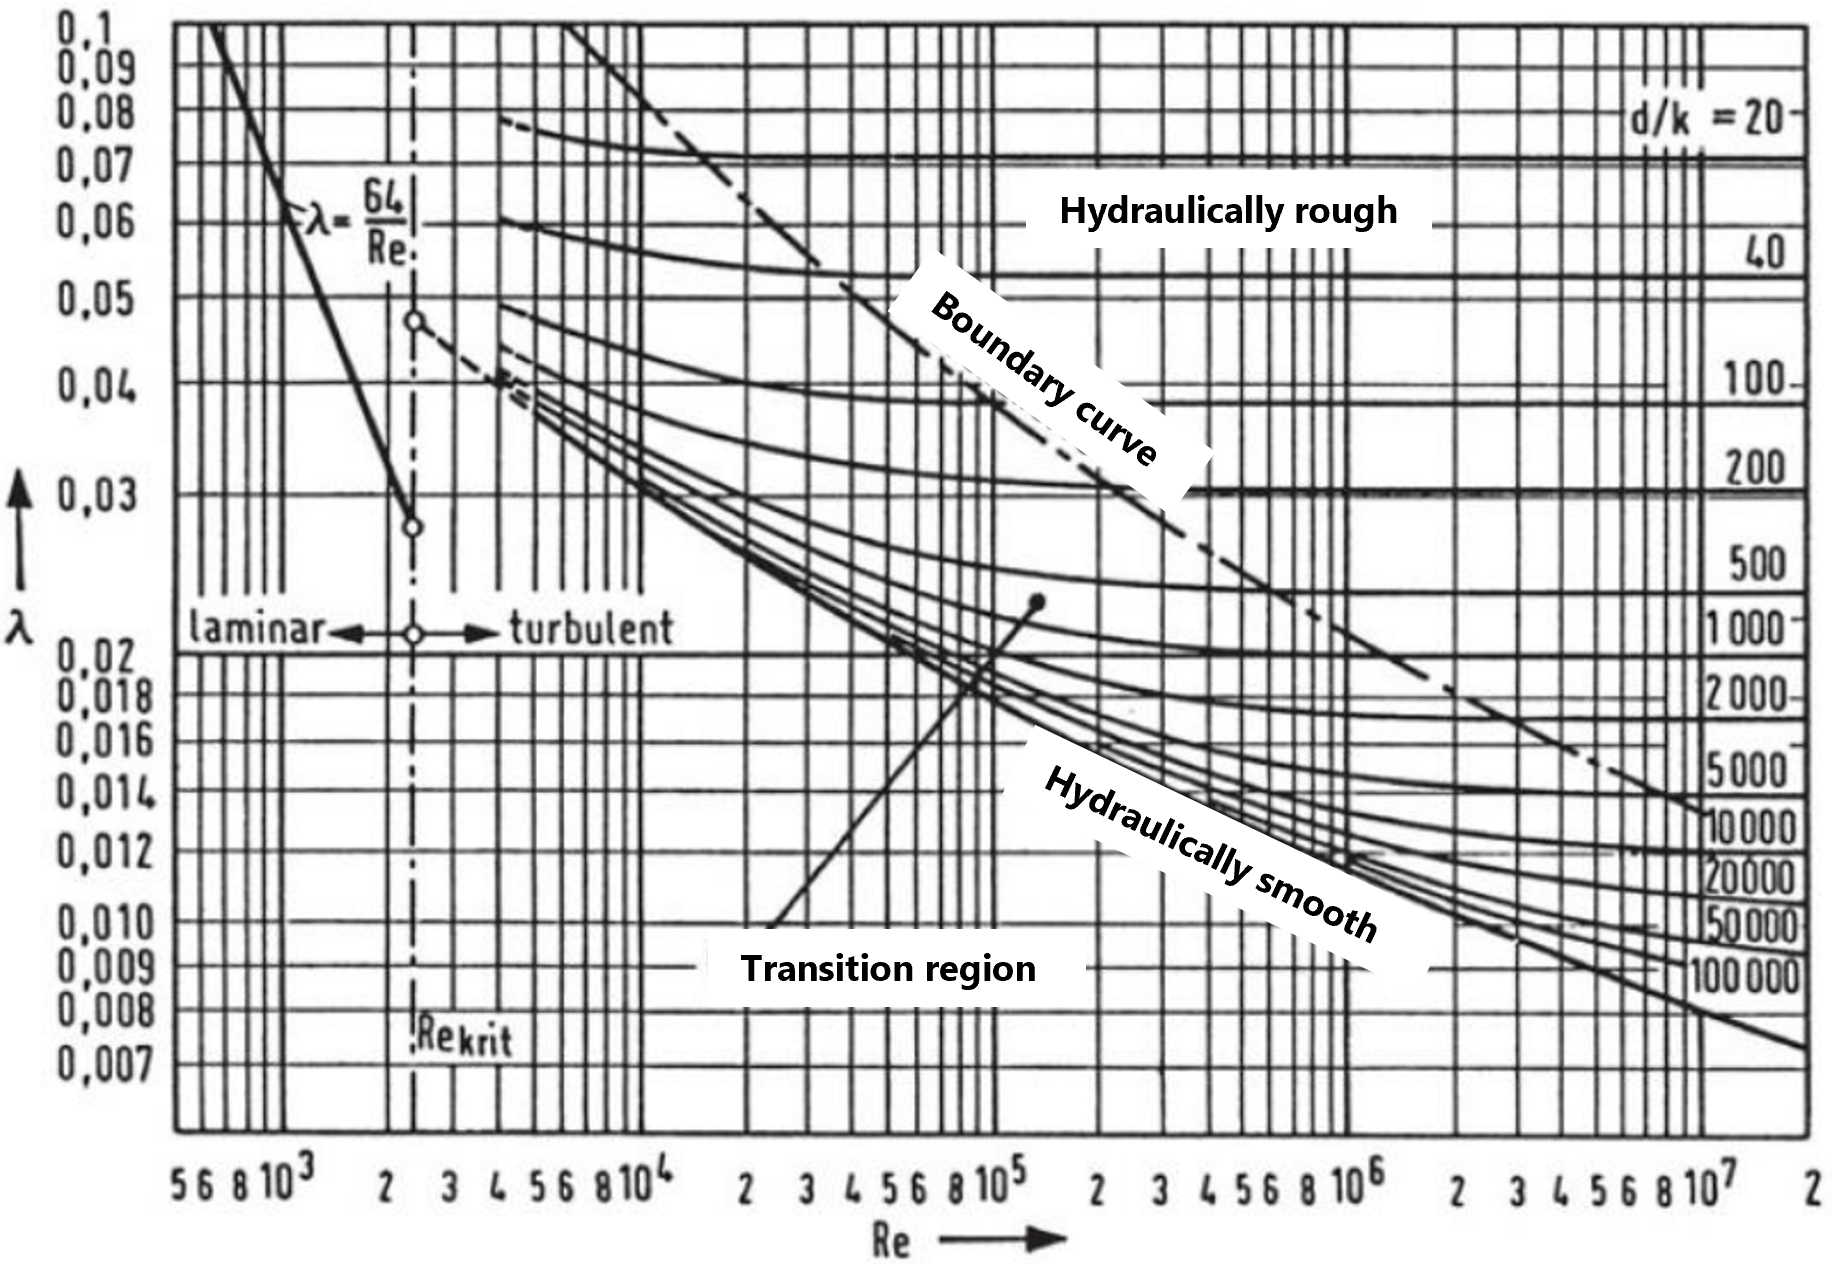
\includegraphics[width=\columnwidth]{media/Moody-Diagramm_en.png}

\begin{theorybox}{Pipe fittings}
    In pipeline systems, a portion of the pressure losses is caused by fittings:
    \begin{equation}
        \Delta p = \zeta \cdot \rho \cdot \frac{v_m^2}{2}
    \end{equation}

    \subsubsection{Elbows}
    \begin{center}
        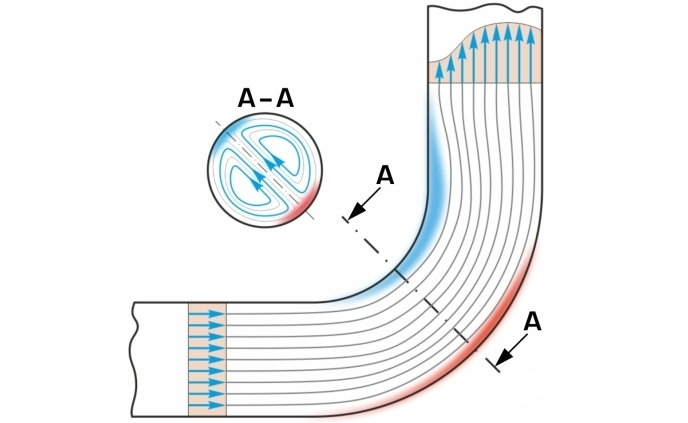
\includegraphics[width=.8\textwidth]{media/Sekundärströmung-Rohrkrümmer.jpg}
    \end{center}
    \begin{align}
        \Delta p = \zeta \cdot \rho \cdot\frac{v^2}{2}\\
        \zeta = f_{Re} \cdot \zeta_u
    \end{align}
    where (given from individual diagrams):
    \begin{itemize}
        \item $\zeta_u$ is the geometric resistance coefficient;
        \item $f_{Re}$ is the Reynolds correction factor.
    \end{itemize}
    
    \subsubsection{Diffuser}
    A diffuser is a section in a pipeline with a continuous increase in cross-sectional area.\\\\
    The frictional losses $\Delta p_v$ in a diffuser are given by:
    \begin{align}
        \Delta p_v &= \frac{\zeta\rho v_1^2}{2}\\
        p_2 - p_1 &= \Delta p_B - \Delta p_v
    \end{align}
    where $\Delta p_B$ is the Bernoulli pressure (frictionless).
\end{theorybox}
\vfill
\phantom{}
\end{multicols}

\newpage
\begin{multicols}{2}
\setlength{\columnsep}{1pt}
\begin{theorybox}{Pipe fittings}
    The diffuser efficiency $\eta_D$ according to Bernoulli:
    \begin{equation}
        \eta_D = \frac{p_2 - p_1}{\Delta p_B} = 1 - \zeta \frac{1}{1 - \left(\frac{A_1}{A_2}\right)^2}
    \end{equation}

    The various coefficients are stated as:
    \begin{align}
        &c_p = \frac{2\left(p_2 - p_1\right)}{\rho v_1^2} = \eta_D \cdot c_{p,id}\\
        &c_{p,id} = 1 - \left(\frac{A_1}{A_2}\right)^2\\
        &\zeta_1 = c_{p,id} - c_p
    \end{align}

    The opening angle of the diffuser can be calculated as:
    \begin{align}
        \tan(\theta) = \frac{d_2 - d_1}{2L}\\
        \varphi = 2\theta
    \end{align}
    The optimal angle $\varphi_{\rm opt}$ is between 6-20 degrees.

    \subsubsection{Inlets and outlets}
\end{theorybox}







\end{multicols}






\end{document}